%%%%%%%%%%%%%%%%%%%%%%%%%%%%%%%%%%%%%%%%%%%%%%%%%%%%%%%%%%%%%%%%%%%%%%%%%%%%%
% Chapter 1: Introducción 
%%%%%%%%%%%%%%%%%%%%%%%%%%%%%%%%%%%%%%%%%%%%%%%%%%%%%%%%%%%%%%%%%%%%%%%%%%%%%%%

En este apartado se van a detallar los diferentes motivos y objetivos a desarrollar, así como la metodología y el plan de trabajo llevado a cabo para la realización del Trabajo de Fin de Grado.

%---------------------------------------------------------------------------------
\section{Motivación}
\label{1:sec:1}

La tecnología con el paso de los años ha ido avanzando a pasos agigantados, de manera que cada día sea más accesible a todas y cada una de las personas que hacen uso de ella en mayor o menor medida. Esto ayuda a que sectores externos a la informática, como la educación, avancen en materia de nuevos conocimientos,
surgiendo así términos como el \textbf{Pensamiento Computacional}.

Podemos entender como pensamiento computacional la capacidad del ser humano para solucionar problemas, crear sistemas y entender de qué manera se comporta el ser humano a través del ámbito de la informática. Este tipo de "pensamiento" beneficia a los estudiantes de todas las edades, adquiriendo la capacidad de abstraer determinados
problemas, que refuerzan y mejoran las habilidades intelectuales, permitiendo que se puedan aplicar en otros ámbitos.

En Internet existen diversas plataformas dedicadas a transmitir el concepto de pensamiento computacional en el ámbito educativo, como son Code.org\cite{Code.org}, Codecademy\cite{Codecademy}, etc. En este trabajo nos hemos centrado en Code.org, una plataforma diseñada con la intención de permitir que este tipo de pensamiento sea divulgado tanto a alumnos de diferentes
escuelas o institutos, en todas las partes del mundo, al igual que de un amplio rango de edades, de forma que desarrollen esta capacidad a través de las actividades que se disponen en la plataforma.

Debido a que en la aplicación mencionada anteriormente no se muestran los resultados de los tests realizados a los alumnos de manera gráfica, se ha desarrollado una plataforma que simule la representación de dichos datos de los estudiantes. Esto permite que se manifieste visualmente en qué medida los alumnos están adquiriendo los conceptos
que se intentan transmitir con los cursos o talleres propuestos en Code.org. 

%---------------------------------------------------------------------------------
\section{Objetivos}
\label{1:sec:2}

Puesto que Code.org ha sido la plataforma elegida para llevar a cabo el proyecto, el objetivo principal a conseguir es realizar una contribución a su página a través de Github, plataforma donde tienen alojada Code.org, de forma que los profesores no sólo tengan los resultados de los alumnos en los cursos impartidos, sino también la posibilidad de
observarlos de manera gráfica, permitiendo ver el progreso de sus alumnos.

En caso de no conseguir dicho hito, se realizará un servicio externo, con la intención de plasmar los datos de los alumnos en gráficas representativas. Dicho servicio simulará la plataforma de Code.org, donde un profesor registrará a los estudiantes en los diferentes cursos o talleres, y podrá observar gráficos filtrados por edades, sexo, niveles completados, etc,
complementando así el servicio que ofrece la plataforma de Code.org.

%---------------------------------------------------------------------------------
\section{Metodología y plan de trabajo}
\label{1:sec:3}

Para desarrollar el proyecto, se ha seguido un plan de trabajo que podría dividirse en diferentes etapas:

\begin{itemize}
  \item Una primera fase, en la que se ha realizado un estudio de los beneficios que supone el aprendizaje del pensamiento computacional en el sector educativo, a través del movimiento global \textbf{Horas de Código}\cite{HourOfCode}, unos talleres impartidos a alumnos en un amplio rango de edad, con la intención de fomentar el aprendizaje del pensamiento computacional.
  \item A continuación, se procedió a valorar las principales páginas (Code.org, Codecademy, Programamos\cite{Programamos}) dedicadas a plasmar este tipo de pensamiento en sus actividades. En última instancia, se decidió que Code.org era la más adecuada para realizar la contribución a los resultados.
  \item Debido a que se actualizaba constantemente el repositorio de Code.org, con su consiguiente cambio en la estructura, se procedió a realizar una plataforma alternativa que intentara simular el funcionamiento de Code.org, con la particularidad añadida de la representación gráfica.
\end{itemize}

El resto de la memoria cuenta con un capítulo que aúna los antecedentes y estado actual del tema con respecto al pensamiento computacional, donde se abordará la explicación de algunas de las plataformas similares a la desarrollada para el proyecto. En el capítulo 3 se explican las diferentes tecnologías utilizadas para realizar el proyecto final, complementando así
al capítulo 4, en el que se expone tanto la arquitectura como el funcionamiento en detalle de la aplicación (CodeCharts). A continuación, en el apartado 5, algunas de las pruebas y verificaciones usadas para el testeo de la plataforma

%------------------------------------------------------------------------------
%\begin{figure}[!th]
%\begin{center}
%\includegraphics[width=0.5\textwidth]{images/arbolbinario.eps}
%\caption{Ejemplo}
%\label{fig:ArbolBinario}
%\end{center}
%\end{figure}
%------------------------------------------------------------------------------

